\documentclass{article} % For LaTeX2e
\usepackage{iclr2027_conference,times}

% Optional math commands from https://github.com/goodfeli/dlbook_notation.
\input{math_commands.tex}

\usepackage{hyperref}
\usepackage{url}
\usepackage{amsmath}
\usepackage{amssymb}
\usepackage{booktabs}
\usepackage{graphicx}
\usepackage[section]{placeins}

\title{Can the Camera Tell? \\ Action-Set Identifiability and Principled
Abstention for Physical 3D Geometry}

% Authors must not appear in the submitted version. They should be hidden
% as long as the \iclrfinalcopy macro remains commented out below.
% Non-anonymous submissions will be rejected without review.
\author{Anonymous authors \\ Paper under double-blind review}

\newcommand{\fix}{\marginpar{FIX}}
\newcommand{\new}{\marginpar{NEW}}

% The paper is float-heavy and the LaTeX defaults leave wide bands of white
% above and below every float; these lengths tighten that without touching
% the ICLR type area.
\setlength{\floatsep}{6pt plus 2pt minus 2pt}
\setlength{\textfloatsep}{8pt plus 2pt minus 2pt}
\setlength{\intextsep}{7pt plus 2pt minus 2pt}
\setlength{\abovecaptionskip}{4pt}
\setlength{\belowcaptionskip}{2pt}
\setlength{\abovedisplayskip}{5pt plus 2pt minus 2pt}
\setlength{\belowdisplayskip}{5pt plus 2pt minus 2pt}
\setlength{\abovedisplayshortskip}{3pt}
\setlength{\belowdisplayshortskip}{3pt}
\renewcommand{\arraystretch}{1.02}
% Allow floats to fill more of a page before LaTeX defers them to a page of
% their own, which is what strands figures among blank space.
\renewcommand{\topfraction}{0.92}
\renewcommand{\bottomfraction}{0.75}
\renewcommand{\textfraction}{0.07}
\renewcommand{\floatpagefraction}{0.85}

%\iclrfinalcopy % Uncomment for camera-ready version, but NOT for submission.
\begin{document}

\maketitle

\begin{abstract}
A corridor seen through a doorway, the same corridor reflected in a mirror, and a
photograph of it shown on a screen can produce the same image. The three differ in
what a hand would touch, so a depth predictor answering from one viewpoint is
guessing between them rather than measuring. This paper asks a prior question:
given the camera motions an observer can perform, is the physical explanation
recoverable at all? We define the separability of two explanations as how
differently they predict the scene will look after a given motion, call a scene
identifiable when some available motion separates every explanation still in play,
and abstain otherwise. On a benchmark whose competing explanations are
pixel-identical at the starting view, abstention drives false physical certainty
from $0.832$ to $0.000$, and choosing interventions on the weakest contending pair
reaches committed accuracy $1.000$ on all four mechanisms where a belief-weighted
sum reaches $0.587$ on mirrors. On real photographs we evaluate twelve published
checkpoints across six architecture families and a $38\times$ parameter range:
every one is fooled on $59.5$--$78.4\%$ of images, the newest family among the most
affected, and on every one the model's own confidence scores \emph{below chance} at
predicting its own failure. Conformal prediction meets its coverage guarantee and
still cannot repair this, since coverage constrains how many predictions are kept
and never which. Selecting the viewpoint at which some hypothesis best explains the
observation cuts error inside the ambiguous region by $31.6\%$ on $12$ of $12$
checkpoints, and a policy reading a \emph{frozen} encoder's features predicts that
encoder's failures better than ten hand-designed quantities and transfers to $12$
of $12$ unseen architectures: the evidence is already in the representation and is
discarded before the output.
\end{abstract}

\section{Introduction}
\label{sec:introduction}

A corridor viewed through an open doorway, the same corridor reflected in a
planar mirror, and a photograph of it displayed on a screen can be arranged to
produce an identical image. The three scenes differ in the surface a hand would
touch, which is empty air in the first case, a pane of glass in the second and a
rigid panel in the third, yet at a single viewpoint the light reaching the sensor
is the same. The physical explanation of the observed geometry is therefore not
determined by the image, and any answer produced from that image alone is
selected by a prior rather than by evidence.

This distinction carries practical weight wherever perception is coupled to
action. A service robot must separate a doorway from its reflection before a path
is committed, an assistive system is expected to report the surface in front of a
user rather than the scene depicted on it, and an augmented-reality device places
content on a panel rather than inside the room that panel shows. In each case the
cost of an error is set by physical contact, so the quantity of interest is the
geometry of the first real surface along the ray, and the failure of interest is a
confident report of geometry that is not present.

\paragraph{From accurate depth to identifiable depth.}
Monocular depth estimation now recovers relative geometry reliably across diverse
scenes, and large pre-trained predictors transfer to unfamiliar imagery with
little adaptation. Several complementary lines of work extend perception to
exactly the configurations described above. Multi-layer and order-aware
formulations represent more than one surface along a ray, so that a transparent
interface and the scene behind it are both retained. Dedicated detectors recover
mirrors and glass as first-class scene elements. Active and next-best-view
perception treats observer motion as a resource to be allocated toward informative
viewpoints. Uncertainty estimation supplies a scalar that accompanies each
prediction, selective prediction converts such a scalar into a decision to answer
or to defer, and split conformal prediction supplies finite-sample guarantees on
how often deferral occurs.

Each of these establishes a capability on which the present work depends, and
together they address what the depth is, which surfaces are present, where the
camera should move next, and how certain a prediction is. The matched
configurations above raise a further question, which is the subject of this paper:
is the physical explanation of this visual geometry recoverable at all from the
observations that this observer is able to make?

\paragraph{Why this is a distinct question.}
Accuracy is a property of a prediction and uncertainty is a property of a
predictor, whereas identifiability is a property of the triple formed by the
competing physical explanations, the actions available to the observer, and the
resolution at which differences become perceptible. A view-tracked display
observed within its aperture is geometrically indistinguishable from the scene it
depicts, and a static planar mirror reflecting a static room produces content
parallax matching that of a real room seen through an opening of the same shape.
In both cases the answer is not merely difficult to obtain, but absent from the
available evidence. Enlarging a model or collecting further images from the same
viewpoint leaves the situation unchanged, whereas a suitable change of viewpoint
resolves it immediately. Identifiability is defined here relative to an action
set for this reason, and the label ``not identifiable'' is treated as a statement
about that triple rather than as a further physical hypothesis. The framing
yields a prediction that can be tested independently of architecture: where the
evidence cannot decide, a scalar confidence has no mechanism by which to register
the absence of evidence, because the same image remains consistent with every
hypothesis.

\paragraph{Contributions.}
\begin{enumerate}\itemsep2pt
\item \textbf{Action-set identifiability as a decision rule.} Separability between
two image-formation hypotheses is defined as the distance between the consequences
they predict for an intervention, and identifiability as the best such separability
attainable over an available action set. Falling below a perceptual threshold
licenses abstention, which turns recoverability into an explicit and computable
precondition for answering.

\item \textbf{A matched-counterfactual benchmark whose premise is measured rather
than assumed.} Competing mechanisms are pixel-identical at the reference view to a
maximum deviation of order $10^{-14}$~px, so chance-level single-view performance
is a verified property of the construction. Cases that no permitted action
resolves are included by design, which makes correct abstention a scorable outcome.

\item \textbf{A weakest-pair criterion for selecting the intervention.} Actions
are chosen to maximise the smallest separability among hypothesis pairs still in
contention, rather than a belief-weighted sum over all pairs. The criterion is
$T$-optimality from optimal design for model discrimination
\citep{atkinson1975design,hunter1965experimental}, applied here to active visual
perception and compared against the summed objective on this problem class.

\item \textbf{A protocol for real photographs, and the ground-truth admissibility
criterion it requires.} Calibrated stereo is treated as a one-element action set,
predictions are calibrated outside the ambiguous region and scored inside it, and
images whose reference measurement cannot arbitrate the question are identified
and excluded.

\item \textbf{Evidence across model families, and a decodable signal.} Behaviour
is characterised over published checkpoints spanning several architecture families,
with trivial baselines reported alongside the proposed measures, and a policy
fitted on features pooled from a frozen encoder transfers to held-out
architectures.
\end{enumerate}

\section{Related Work}
\label{sec:related}

\paragraph{Depth on mirrors, glass and displays.}
Mirrors are recovered as first-class scene elements with dedicated instance masks
and plane annotations, enabling depth to be refined on surfaces where standard
reconstruction fails \citep{mirror3d2021}, and transparency is modelled by
decomposing radiance into interface, transmitted and reflected components
\citep{glint2026}. Benchmarks quantify the difficulty directly, covering specular
and transparent surfaces with dense annotation \citep{booster2023}, large-scale
transparent objects \citep{clearpose2022}, and simulation-to-real depth
restoration for such materials \citep{dreds2022}. These establish that the
surfaces studied here are recognised as difficult and that recovering their
geometry is an active target. The present work takes a step back from recovering
the geometry and asks first whether the mechanism producing an appearance is
recoverable from the observations available.

\paragraph{Multi-layer and order-aware geometry.}
Representing more than one surface along a ray is well established. Ordinal
multi-layer benchmarks supply relations for both the first surface and the scene
behind it, together with real and synthetic training data
\citep{layereddepth2025}; self-determined grouping formulates transparency as
unordered events along a ray \citep{seegroup2026}; and steerable predictors
condition on a focus distance to select which layer is returned
\citep{depthfocus2026}. This line supplies the representational capacity that the
present formulation assumes, and one such benchmark is used here as an independent
evaluation set whose annotations share no machinery with the measures defined in
Section~\ref{sec:method}.

\paragraph{Apparent versus physical geometry.}
That predictors report depicted rather than physical structure is documented at
scale by a benchmark spanning illusion categories including printed pictures,
screens and mirrors \citep{illusion2025}. The distinction between apparent and
physical geometry is therefore taken as established. What is added here is a
criterion determining when that distinction is decidable from the observations an
observer can obtain, together with an explicit abstention when it is not, and a
benchmark constructed so that such undecidable cases are present and scorable.

\paragraph{Active perception and experimental design.}
Selecting viewpoints to maximise expected information is long established in
active and next-best-view perception, where the objective is typically a
belief-weighted sum over competing possibilities. The question posed here is
complementary: rather than which view is most informative, it asks whether any
view within a bounded action set is informative enough to license a commitment.
The criterion used for that purpose is not new. Designing experiments to
discriminate between rival models is a mature area of statistics, in which the
maximin criterion of \eqref{eq:maximin} is known as $T$-optimality
\citep{atkinson1975design,hunter1965experimental}; its role here is the transfer
of that criterion into active visual perception.

\paragraph{Causal identifiability, selective and conformal prediction.}
Identifiability under temporal interventions is established in causal
representation learning \citep{citris2022}; that interventional framing is
borrowed and applied to the narrower question of which optical mechanism produced
an image, with the action set playing the role of the intervention family.
Deferring on uncertain inputs follows Chow's rule \citep{chow1970}, and split
conformal prediction supplies distribution-free, finite-sample coverage guarantees
\citep{vovk2005,lei2018}. Those guarantees constrain how many predictions are
retained rather than which ones, so a calibrated procedure inherits the ranking of
the score it wraps. The abstention rule used here is derived instead from a
geometric condition on the available evidence, and conformal prediction is retained
as a baseline against which that condition is compared.

\section{Method}
\label{sec:method}

The method keeps a set of competing physical explanations for an observed image,
predicts what each implies after a candidate camera motion, measures how far those
predictions diverge, and answers only when some available motion is guaranteed to
separate every explanation still in contention.

\begin{figure}[t]
\begin{center}
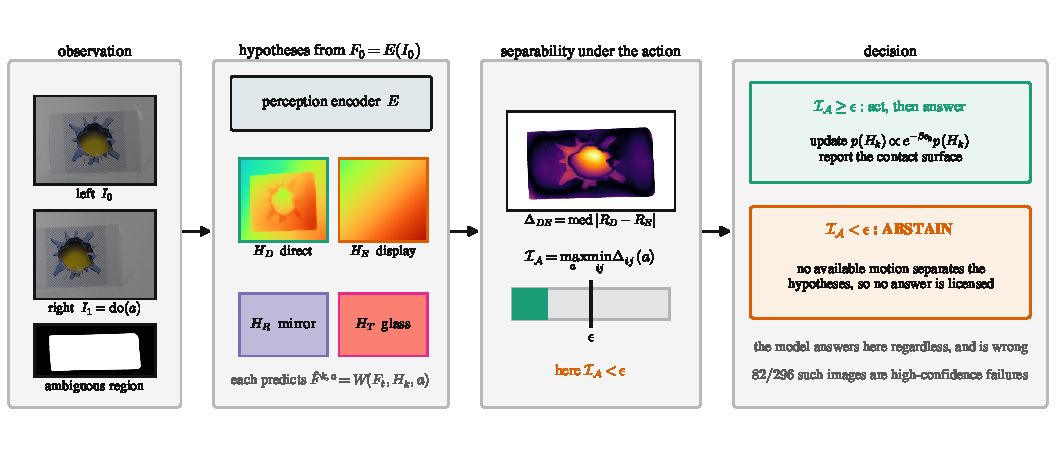
\includegraphics[width=\linewidth]{figures/fig_system.pdf}
\end{center}
\caption{\textbf{The method on one real image.} A stereo pair supplies an executed
action, and the annotated region marks where the surface is ambiguous. The
encoder's geometry gives $H_D$ directly and, fitted to a plane over the same
region, $H_E$; mirror and glass enter the same way where the scene admits them.
Warping the second view under each hypothesis gives the separability $\Delta_{DE}$
of \eqref{eq:delta-photometric}, and identifiability \eqref{eq:identifiability} is
compared against the perceptual threshold. It lies below it, so
\eqref{eq:abstain} correctly declines to answer on a scene no available motion
resolves, while the predictor answers and is wrong.
Depth maps are from a published checkpoint used as released.}
\label{fig:system}
\end{figure}

\subsection{Hypotheses and the action set}
\label{sec:formulation}

Let $I_0$ be an image at reference pose $C_0$ and $F_0 = E(I_0)$ the geometry a
perception encoder $E$ reports for it, as landmarks carrying image coordinates,
depths and visibility flags. Rather than returning $F_0$ alone, a family of
image-formation hypotheses is kept: $H_D$ asserts the structure is physically
present, $H_E$ that it is depicted on a flat emissive panel, $H_R$ that it is a
virtual image in a planar mirror, and $H_T$ that it is seen through a planar
transparent slab. Each places the first touchable surface elsewhere, which is the
distinction a contact-based cost makes. They are matched by construction, being
pixel-identical at $C_0$, so any later gain from moving the camera is attributable
to the motion rather than to a residual appearance difference.

The observer acts. An action $a \in SE(3)$ is a rigid camera motion applied as an
explicit intervention,
\begin{equation}
\label{eq:intervention}
\mathrm{do}\!\left(C_1 = C_0 \cdot a\right),
\end{equation}
where $C_0$ is the reference pose, $C_1$ the resulting pose and $\cdot$ composition
of rigid transforms. The $\mathrm{do}(\cdot)$ notation replaces conditioning
because the viewpoint is chosen rather than encountered, so the evidence is
attributable to the action. Actions come from a bounded, enumerable set $\mathcal{A}$: translations of
$\{0.05, 0.10, 0.20, 0.30\}$~m along three axes and rotations of
$\{5^\circ, 10^\circ\}$ in yaw and pitch, both directions, plus the null action,
giving $|\mathcal{A}| = 33$ under a budget of $0.35$~m and $15^\circ$. The budget is
modest because the setting is a device making a small corrective movement rather
than one repositioning freely. Finiteness lets identifiability be evaluated by
enumeration before any motion, which is what makes abstention possible in advance
of acting. Landmarks are the encoder's own output sampled on a fixed grid over the
scene, each carrying an image coordinate, a depth and a visibility flag; visibility
under a hypothesis is decided by z-buffering that hypothesis' predicted geometry,
so a landmark occluded under one mechanism and not another contributes to
$D_{\text{occlusion}}$.

\subsection{Predicting the consequence of an action}
\label{sec:transition}

Each hypothesis maps current geometry and a candidate action to a predicted
observation,
\begin{equation}
\label{eq:transition}
\hat{F}^{\,k,a} \;=\; W\!\left(F_t,\, H_k,\, a\right),
\end{equation}
where $F_t$ is the geometry at time $t$, $H_k$ the $k$-th hypothesis, $a$ the
candidate action and $\hat{F}^{\,k,a}$ what $H_k$ predicts after executing $a$. The
transition $W$ applies one shared projection to every hypothesis and differs only
in the world each asserts: a panel paints content on the screen plane, gaining no
differential parallax; a mirror keeps the parallax of virtual structure while
adding moving virtual images of observer-attached markers; a slab displaces content
axially. Sharing the projection makes any difference between predictions
attributable to the mechanism rather than to rendering.

The mechanisms are planar for a reason the construction depends on. A planar
mirror reflects exactly across a plane and a planar slab displaces content
axially by $d\,(1 - 1/n)$, so each transition is closed form. That is what makes the counterfactuals \emph{matched}: reference views can be
made pixel-identical to numerical precision, and any divergence after an action
is attributable to the mechanism rather than to approximation error. A curved
surface admits no exact transition, and a learned one would reintroduce the
confound the shared projection removes. The restriction is a condition for the
experiment to be clean rather than a limit of the formalism, which is
independent of it (Appendix~\ref{sec:supp-extension}).

\subsection{Separability, identifiability and abstention}
\label{sec:separability}

Pairwise separability is the distance between the consequences two hypotheses
predict for the same action,
\begin{equation}
\label{eq:separability}
\Delta_{ij}(a) \;=\; D\!\left(\hat{F}^{\,i,a},\, \hat{F}^{\,j,a}\right),
\end{equation}
where $i,j$ index two hypotheses and $D$ is a composite distance,
\begin{equation}
\label{eq:distance}
D \;=\; \lambda_m D_{\text{motion}} + \lambda_o D_{\text{occlusion}}
      + \lambda_g D_{\text{geometry}} + \lambda_f D_{\text{feature}} .
\end{equation}
Here $D_{\text{motion}}$ is the root-mean-square image-space displacement between
the two predicted landmark sets over jointly visible landmarks, in pixels;
$D_{\text{occlusion}}$ counts landmarks whose predicted visibility differs;
$D_{\text{geometry}}$ is the root-mean-square 3-D distance between back-projected
landmarks; $D_{\text{feature}}$ is reserved for a learned feature distance; and
$\lambda_m, \lambda_o, \lambda_g, \lambda_f$ weight them. Throughout
$\lambda_m = 1$, $\lambda_o = 4.0$~px per disagreeing landmark, and
$\lambda_g = \lambda_f = 0$, placing $D$ in pixels so the threshold below is a
perceptual displacement threshold in the same units. The occlusion term counts
rather than takes a fraction, since a fraction would be diluted by the landmark
count; its weight places one unambiguous appearance or disappearance clearly above
the $1$~px threshold, which matters because that is frequently the only cue a
mirror offers. Priors over hypotheses are uniform at $t = 0$. The sensitivity of
the decision to $\epsilon$ and to the admissibility criterion is reported in
Appendix~\ref{sec:supp-sensitivity}.

The quantity of interest is the best separability the action set attains,
\begin{equation}
\label{eq:identifiability}
\mathcal{I}_{\mathcal{A}}\!\left(H_i, H_j\right)
\;=\; \max_{a \in \mathcal{A}} \; \Delta_{ij}(a),
\end{equation}
so a pair counts as separable if any single permitted motion would distinguish it.
The system abstains when
\begin{equation}
\label{eq:abstain}
\min_{(i,j)} \; \mathcal{I}_{\mathcal{A}}\!\left(H_i, H_j\right) \;<\; \epsilon ,
\end{equation}
the minimum running over pairs still in contention. The order matters: a maximum
over actions inside a minimum over pairs licenses an answer only if some action
separates every undecided pair, since the pair left unseparated is exactly where an
error would be made. The threshold is fixed at $\epsilon = 1.0$~px and not tuned,
being a property of the sensor and the perceptual criterion: altering it changes
what ``identifiable'' denotes and relabels the benchmark rather than improving
performance on it.

\subsection{Choosing the intervention}
\label{sec:selection}

Two objectives are compared. The first is the summed objective standard in active
perception,
\begin{equation}
\label{eq:sum}
a^{\star}_{\text{sum}} \;=\; \arg\max_{a \in \mathcal{A}}
\;\sum_{i<j} p_i\, p_j\, \Delta_{ij}(a),
\end{equation}
where $p_i, p_j$ are posterior probabilities, so still-plausible pairs contribute
more. Such a sum can be maximised by an action separating pairs not in contention
while leaving the deciding pair unseparated, since a large term compensates for a
zero one. The second replaces the sum with the weakest contending pair,
\begin{equation}
\label{eq:maximin}
a^{\star}_{\text{maximin}} \;=\; \arg\max_{a \in \mathcal{A}}
\;\min_{(i,j) \in \mathcal{C}} \; w_{ij}\, \Delta_{ij}(a),
\end{equation}
where $\mathcal{C}$ collects pairs whose joint posterior mass has not collapsed and
$w_{ij}$ weights each by that mass. The form follows from the abstention rule: a
decision needs every contending pair separated, so the binding quantity is the
smallest separability rather than the sum. This is $T$-optimality from optimal
design for model discrimination
\citep{atkinson1975design,hunter1965experimental}, applied to active vision.

\paragraph{Which quantity is available, and when.}
Both objectives are stated over hypothesis \emph{pairs} and so need at least two
pairs to differ. Four mechanisms give six pairs in the synthetic benchmark, where
the weakest-pair form is the operative criterion. A calibrated stereo pair supports
two mechanisms and hence one pair, so on real photographs \eqref{eq:sum} and
\eqref{eq:maximin} coincide. Selection there runs instead through the belief update
of \eqref{eq:belief}: among viewpoints the observer could occupy, prefer the one at
which some hypothesis best accounts for the view actually obtained,
\begin{equation}
\label{eq:evidence-selection}
a^{\star}_{\text{evidence}} \;=\; \arg\min_{a \in \mathcal{A}} \;
\min_{k} \; e_k(a),
\end{equation}
with $e_k(a)$ the residual of hypothesis $k$ after executing $a$. Both rules act on
the same belief machinery, one through the separability entering it and one through
the residual leaving it, and each is used where the evidence it needs exists.

\subsection{Belief update and output}
\label{sec:belief}

After the selected action is executed and $O'$ observed, each hypothesis has
residual $e_k = D(\hat{F}^{\,k,a^\star}, E(O'))$ under the same
distance~\eqref{eq:distance}, so prediction error and separability share a scale.
Belief updates multiplicatively,
\begin{equation}
\label{eq:belief}
p_{t+1}(H_k) \;\propto\; \exp\!\left(-\beta\, e_k\right)\, p_t(H_k),
\end{equation}
where $p_t(H_k)$ is the prior mass on hypothesis $k$, $e_k$ its residual in pixels
and $\beta$ converts error into log-likelihood; $\beta = 1.0$ makes a one-pixel
error cost one nat. A posterior floor stops one unlucky observation eliminating a
hypothesis permanently. The system then names the mechanism and reports its contact
geometry, the first physical surface along each ray, which is the glass for a
mirror and the panel for a display. Commitment is withheld when the posterior
maximum does not exceed $\tau = 0.45$, set just below the $0.5$ tie a forced choice
over a two-way ambiguity produces, so such a choice counts as false certainty
rather than caution.

\subsection{Benchmark and metrics}
\label{sec:benchmark}

Each base scene is instantiated under every mechanism with content adjusted so the
reference views coincide, to a maximum deviation of order $10^{-14}$~px, making
chance-level single-view performance a verified property rather than an assumption.
Configurations no permitted action resolves, namely view-tracked displays within
their aperture and mirrors mimicking an opening, are included deliberately: without
them a method that never abstains would be indistinguishable from one that abstains
correctly. Splits are formed by base scene.

Four quantities are reported. Causal explanation accuracy (CEA) is
$P(\hat{H} = H^\star)$ with abstention counted as an error, and committed accuracy
is $P(\hat{H} = H^\star \mid \text{answered})$; the first penalises caution and the
second rewards it, so together they expose the trade between answering and being
right. False physical certainty (FPCR) is
$P(\max_k p(H_k) > \tau \mid y_{\mathrm{id}} = 0)$, measured only on unresolvable
cases, and is what abstention exists to reduce. Normalised regret compares the
chosen action's utility against the best available.

\subsection{Protocol for real photographs}
\label{sec:real-protocol}

A calibrated rectified stereo pair supplies one executed action with known
parameters, the baseline translation, so real data is the case $|\mathcal{A}| = 1$.
Four elements stop the measurement absorbing the effect under study.

\textbf{Calibration outside, scoring inside.} A monocular predictor returns
relative inverse depth, defined up to unknown scale $s$ and shift $t$, fitted by
least squares against reference disparity on the non-ambiguous region and applied
inside it, giving the disparity predicted under $H_D$,
\begin{equation}
\label{eq:align}
d_{D} \;=\; s\,\hat{p} + t ,
\end{equation}
with $\hat{p}$ the raw prediction. Determining the two parameters where the
predictor performs well stops them absorbing the discrepancy under study. The
disparity under $H_E$ is the least-squares plane through $d_D$ over that region,
fitted to the prediction and never the reference, which would place ground truth
inside a quantity that must be computable at test time.

\textbf{Separability is measured photometrically.} The right image is warped into
the left frame under each hypothesis, using the rectified-stereo relation that
column $x$ with disparity $d$ corresponds to column $x - d$ in the other view,
\begin{equation}
\label{eq:warp}
R_{k}(x, y) \;=\; I_{\text{right}}\!\left(x - d_{k}(x,y),\; y\right),
\qquad k \in \{D, E\},
\end{equation}
and separability is the median absolute difference between the two warps inside the
region,
\begin{equation}
\label{eq:delta-photometric}
\Delta_{DE} \;=\; \operatorname{median}\left|R_{D} - R_{E}\right| .
\end{equation}
Both terms warp the same photograph, so illumination, sensor noise and
rectification error appear in both and cancel. Intensity units are deliberate: a
disparity disagreement is visible only where the image carries structure to reveal
it, so on a featureless region two hypotheses predict different geometry and
identical pixels, and the scene is unidentifiable at any baseline.

\textbf{Ground truth is admitted only when it can arbitrate.} A printed sheet or
panel is flat, so reference disparity inside the region should be planar. Where it
is not, stereo matching has locked onto displayed content rather than the panel and
cannot settle what the predictor reported. An image is retained only when a plane
fitted to that disparity attains $R^2 \geq 0.90$, and the number excluded is
reported.

\textbf{Failure is defined without reference to any signal under test.} A predictor
is recorded as fooled when its relative error inside the region exceeds its error
outside, a label mentioning neither confidence nor identifiability. Quantities
requiring no model and no theory, including the fraction of the frame the region
occupies, are reported alongside the proposed measures so any advantage is visible
against them. All AUROC values use the convention that a larger score indicates
greater likelihood of error, so a value below $0.5$ appears as anti-correlation
rather than being concealed by inverting the score. A second dataset supplies
ordinal relations between point pairs together with a per-point layer index
authored independently of this work, an external label of ambiguity sharing no
machinery with the measures above.

\subsection{Learned abstention and models evaluated}
\label{sec:learned}

Two policies are evaluated, both leaving the predictor frozen and fitting only a
small model on top, since the predictor's behaviour is the object of study. The
first uses the hand-designed quantities above. The second pools the network's own
frozen intermediate features over the ambiguous region, keeping the difference
between the pooled representation inside and outside it plus the within-region
spread; the contrast is used because a representation encoding ambiguity should
differ inside the region relative to its surroundings, whereas an absolute vector
would largely encode which scene is viewed. Three classifier families are fitted so
the result does not rest on one inductive bias: $L_2$-regularised logistic
regression, histogram gradient boosting and \textsc{XGBoost}, the boosted models
held to depth $3$ with at least $40$ samples per leaf, since a few thousand rows
over fewer than a hundred scenes would otherwise be memorised.

Three protocol choices make these interpretable. Folds are split by base scene,
because the benchmarks photograph one scene from several viewpoints and a random
split would report memorisation as transfer. Leave-one-model-out trains on all
checkpoints but one and tests on the held-out one, asking whether failure is
predictable as a property of the image rather than of one network. Hyperparameter
selection is nested, with settings chosen on inner folds and scored only on outer
folds unseen during selection, since a single-level sweep reporting its own best
score would be optimistically biased by more than the margin claimed.

Published checkpoints are used as released, spanning six architecture families and
a $38\times$ range in parameter count, with nothing trained or tuned on any
evaluation set. One detail affects correctness: the attribute conventionally named
\texttt{predicted\_depth} carries metric depth in some families and inverse depth
in others, so each checkpoint's convention is verified against reference stereo
disparity before use; an inverted convention would exchange near for far while
still producing plausible numbers.

\section{Results}
\label{sec:results}

\begin{figure}[t]
\begin{center}
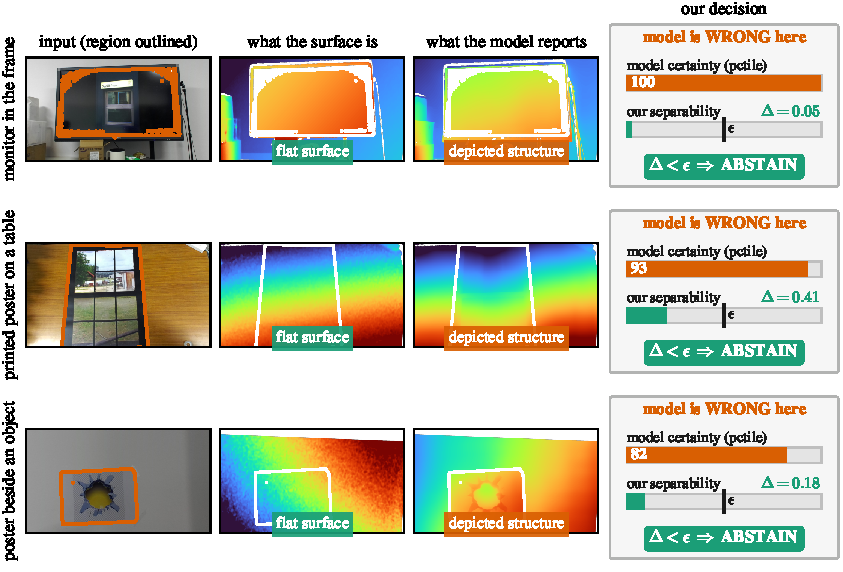
\includegraphics[width=0.88\linewidth]{figures/fig_qualitative.pdf}
\end{center}
\caption{\textbf{Why the decision is needed.} Each row is an image the model gets
wrong: the reference shows a flat sheet or panel, the model reports the structure
depicted on it. Being wrong costs it no certainty, and in the top row it is the
most confident prediction of all $296$ images. The separability $\Delta$ available
from the executed motion falls below $\epsilon$ in every case, so \eqref{eq:abstain}
declines to answer. Across the benchmark $82$ of $296$ images are failures where the
model ranks in the most-confident $30\%$ and this rule abstains.}
\label{fig:qualitative}
\end{figure}

\subsection{Synthetic benchmark}
\label{sec:res-synth}

Table~\ref{tab:phase1} reports Phase~1 over $11$ seeds with the benchmark redrawn
per seed, so intervals reflect the data-generating process rather than model-side
noise. The single-view classifier sits at exactly chance in every seed, confirming
that the matched construction leaves nothing for a single view to exploit, and the
ordering single-view $<$ passive $<$ intervention-aware holds strictly in $11/11$
seeds individually.

\begin{table}[t]
\caption{\textbf{Phase~1, $11$ seeds, mean $\pm$ std, chance $0.333$.} CEA scores
abstention as an error, so committed accuracy is the like-for-like column. Removing
hypothesis conditioning collapses every separability to zero and the system
abstains everywhere, the correct failure mode for a load-bearing component.}
\label{tab:phase1}
\begin{center}
\footnotesize
\begin{tabular}{lccccc}
\toprule
\textbf{Method} & \textbf{CEA} & \textbf{Committed} & \textbf{Abst.} &
\textbf{AUROC} & \textbf{FPCR} \\
\midrule
Single-view classifier    & $0.333{\pm}0.000$ & $0.333{\pm}0.000$ & $0\%$  & $0.505{\pm}0.066$ & $0.000{\pm}0.000$ \\
Passive multi-view        & $0.621{\pm}0.046$ & $0.621{\pm}0.046$ & $0\%$  & $0.748{\pm}0.065$ & $0.868{\pm}0.107$ \\
Generic NBV proxy         & $0.371{\pm}0.050$ & $0.706{\pm}0.029$ & $48\%$ & $0.898{\pm}0.026$ & $0.000{\pm}0.000$ \\
Random intervention       & $0.409{\pm}0.056$ & $0.730{\pm}0.027$ & $44\%$ & $0.925{\pm}0.024$ & $0.000{\pm}0.000$ \\
Max-baseline intervention & $0.502{\pm}0.061$ & $0.824{\pm}0.019$ & $39\%$ & $0.963{\pm}0.028$ & $0.000{\pm}0.000$ \\
\midrule
\emph{abl.}\ no hypothesis cond. & $0.000{\pm}0.000$ & --- & $100\%$ & $0.500{\pm}0.000$ & $0.000{\pm}0.000$ \\
\emph{abl.}\ noisy encoder       & $0.557{\pm}0.034$ & $0.848{\pm}0.049$ & $34\%$ & $0.994{\pm}0.016$ & $0.008{\pm}0.026$ \\
\emph{abl.}\ no abstention       & $\mathbf{0.722{\pm}0.029}$ & $0.722{\pm}0.029$ & $0\%$ & $1.000{\pm}0.000$ & $0.832{\pm}0.107$ \\
\textbf{Ours} & $0.560{\pm}0.032$ & $\mathbf{0.855{\pm}0.054}$ & $34\%$ & $1.000{\pm}0.000$ & $\mathbf{0.000{\pm}0.000}$ \\
\bottomrule
\end{tabular}
\end{center}
\end{table}

Table~\ref{tab:phase2} isolates the choice of intervention. In both studies the
summed objective \eqref{eq:sum} falls short on mirrors while maximin
\eqref{eq:maximin} reaches $1.000$, because a belief-weighted sum can be maximised
by an action that separates pairs not in contention and leaves the deciding pair
unseparated. The gap is structural rather than a threshold choice, since an action
scoring zero on a pair cannot separate it at any $\epsilon$.

\begin{table}[t]
\caption{\textbf{Choosing the intervention, $11$ seeds per study.} Under forced
choice maximin exceeds the passive baseline by $+0.297$ ($t = 41.6$, $11/11$
seeds). Chance is $0.250$ in Phase~2.}
\label{tab:phase2}
\begin{center}
\footnotesize
\begin{tabular}{lccccc}
\toprule
& \multicolumn{2}{c}{\textbf{Mirror committed}} &
\multicolumn{3}{c}{\textbf{Phase~2, four mechanisms}} \\
\cmidrule(lr){2-3}\cmidrule(lr){4-6}
\textbf{Objective} & selector study & Phase~2 & committed & abstains & forced CEA \\
\midrule
Single-view classifier & --- & --- & $0.250{\pm}0.000$ & $0\%$ & $0.250{\pm}0.000$ \\
Passive multi-view     & --- & --- & $0.510{\pm}0.021$ & $0\%$ & $0.510{\pm}0.021$ \\
Max-baseline           & --- & $0.887$ & $0.930{\pm}0.019$ & $73\%$ & --- \\
Summed \eqref{eq:sum}  & $0.587{\pm}0.172$ & $0.956{\pm}0.037$ & $0.986{\pm}0.011$ & $69\%$ & --- \\
\textbf{Maximin} \eqref{eq:maximin} & $\mathbf{1.000{\pm}0.000}$ & $\mathbf{1.000{\pm}0.000}$ & $\mathbf{1.000{\pm}0.000}$ & $72\%$ & $\mathbf{0.808{\pm}0.024}$ \\
\bottomrule
\end{tabular}
\end{center}
\end{table}

\subsection{Real photographs}
\label{sec:res-universal}

Twelve published checkpoints spanning six architecture families and a $38\times$
range in parameter count are evaluated as released
(Figure~\ref{fig:main}a,b; per-checkpoint values in Table~\ref{tab:models}). Every
one is fooled on $59.5$--$78.4\%$ of admissible images, the newest family among the
most affected, and on every one the model's own confidence scores below chance at
predicting its own failure ($0.234$--$0.465$), while identifiability ranges
$0.467$--$0.719$ and exceeds confidence on all twelve.

Calibration cannot repair a signal ordered against the quantity of interest. Both
signals meet their split-conformal coverage guarantee at all five levels tested,
yet deferring on confidence leaves a retained set failing at $76.6\%$ against a
$65.2\%$ base rate, while deferring on identifiability lowers it to $54.4\%$
(Figure~\ref{fig:main}d, Table~\ref{tab:conformal}).

\begin{figure}[!htb]
\begin{center}
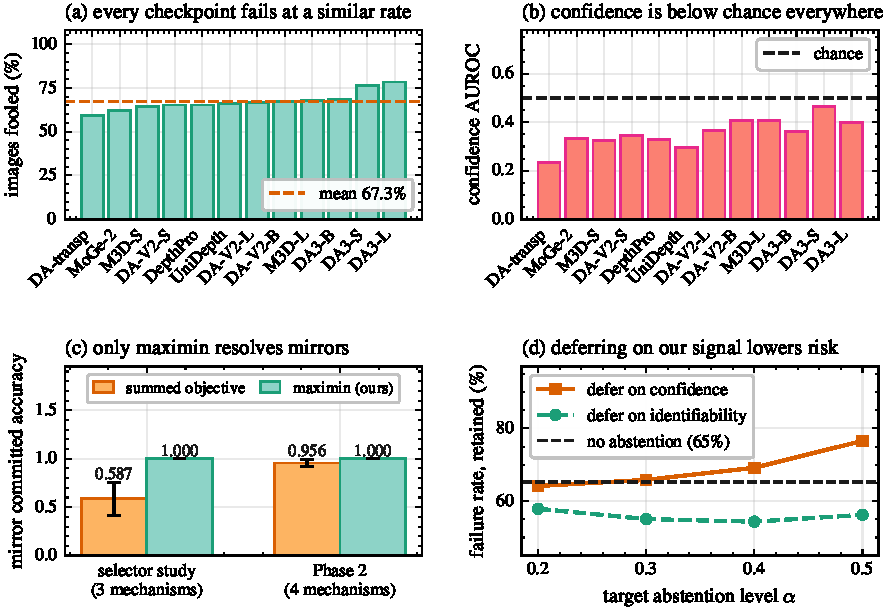
\includegraphics[width=\linewidth]{figures/fig_main.pdf}
\end{center}
\caption{\textbf{Headline results.} (a) The proportion of images each checkpoint is
fooled on stays within a narrow band despite a $38\times$ range in parameter count,
so the behaviour is structural rather than a capacity limitation. (b) Every
checkpoint's own confidence lies below chance at predicting its own failure.
(c) Mirror committed accuracy in both selector studies; only maximin reaches
$1.000$. (d) Split-conformal selective risk: both signals meet coverage, but only
deferring on identifiability lowers the failure rate.}
\label{fig:main}
\end{figure}

Two further measurements support the protocol. The admissibility criterion of
Section~\ref{sec:real-protocol} excludes $159$ of $455$ images whose stereo
reference locks onto displayed content rather than the panel; on admissible images
where a monitor fills the frame, error inside the region is $2.22\times$ that
outside and every image is fooled, with reference planarity $0.989$ against $0.821$
for the prediction. Independently, on a second dataset with ordinal rather than
dense supervision, accuracy split by the benchmark authors' own per-point layer
index gives $0.848$ against $0.737$ across $306{,}874$ pairs, and a second
architecture shows a larger gap still ($0.843$ against $0.669$;
Table~\ref{tab:supp-layered}). That label shares no machinery with any measure
defined here.

\subsection{Choosing where to look, on real photographs}
\label{sec:res-viewpoint}

The benchmark photographs each static scene from several camera positions, and the
median stereo disparity differs across those frames while the scene itself does
not, which is what a moved observer produces. Fifty-five scenes therefore offer a
real action set of three or more viewpoints, and selection can be evaluated on
photographs rather than in simulation. Applying
\eqref{eq:evidence-selection}, and measuring the relative error inside the
ambiguous region so that the outcome depends on no other part of the image,
choosing the best-explained viewpoint reduces that error by $\mathbf{31.6\%}$
relative to choosing uniformly at random, and does so on $\mathbf{12}$ of $12$
checkpoints; the proportion of images on which the predictor is fooled falls from
$48.7\%$ to $44.1\%$, on $9$ of $12$. Table~\ref{tab:supp-viewpoint} gives the full
comparison. What is measured is the error at the chosen viewpoint rather than the
recovery of the mechanism itself, since real images carry no mechanism annotation;
it is the closest test the data supports.

\subsection{Learned abstention}
\label{sec:res-learned}

The signals above are hand-designed, so a natural question is whether a learned
combination does better and whether what it learns is specific to one predictor.
Under leave-one-model-out, a gradient-boosted policy trained on eleven checkpoints
and tested on the twelfth reaches $\mathbf{0.880}$ against $0.764$ for the
strongest single feature, ahead on $\mathbf{12}$ of $12$ held-out checkpoints
(Figure~\ref{fig:transfer}). Nested selection moves that by under $0.01$ and two
boosted families agree within $0.002$, so it is not an artefact of tuning. On a
single checkpoint, where every method sees identical data, a head reading
\emph{frozen} encoder features reaches $\mathbf{0.879}$ against $0.858$ for ten
hand-designed quantities and $0.819$ for the strongest single feature
(Table~\ref{tab:supp-learned}).



\section{Discussion and Conclusion}
\label{sec:discussion}

Making recoverability a precondition for answering, rather than an assumption,
changes what a perception system can be held to, and the measurements bear that
out at both ends. On the synthetic benchmark the single-view classifier sits at
exactly chance in every seed, confirming that the construction leaves nothing for
one view to exploit; abstention then takes false physical certainty from $0.832$ to
$0.000$ while committed accuracy rises from $0.722$ to $0.855$, and choosing
interventions on the weakest contending pair reaches $1.000$ on all four mechanisms
where a belief-weighted sum reaches $0.587$ on mirrors, the case whose deciding
pair a sum can leave unseparated. Selected actions also carry a margin: under
$\pm 1$~cm and $\pm 0.5^{\circ}$ of execution error the selector loses $2.9\%$ of
its accuracy where a hypothesis-blind proxy loses $48.4\%$.

The real-data results are what give the framing its weight. What existing depth
predictors get wrong here is structural rather than a capacity limitation: across
twelve checkpoints spanning six architecture families and a $38\times$ parameter
range, the proportion of images on which they report the depicted scene rather than
the surface stays between $59.5\%$ and $78.4\%$, the newest family among the most
affected, which is what one expects when the information is absent from the input
rather than hard to extract. Confidence is the wrong instrument for it, scoring
below chance on every checkpoint, and calibration cannot repair that: conformal
prediction meets coverage at every level and still retains a set failing more often
than answering everything, since coverage constrains how many predictions are kept
and never which. Three results establish that the ambiguity is nonetheless
tractable. A second benchmark confirms it independently, its authors' own layer
labels giving $0.848$ against $0.737$ across $306{,}874$ pairs on two
architectures. Choosing the viewpoint at which some hypothesis best explains the
observation lowers error inside the region by $31.6\%$ on every checkpoint tested.
And a head fitted to a \emph{frozen} encoder's features predicts that encoder's
failures better than ten hand-designed quantities and transfers to $12$ of $12$
unseen architectures, so what marks these scenes as ambiguous already survives into
the representation and is discarded before the output: a decoding problem rather
than a perception one.

Three points of scope, detailed in the supplement: the synthetic identifiability
AUROC is produced by the procedure that defines its label, so it is read as a
contrast against the classifiers; abstention removes false physical certainty
entirely in the clean configuration and in ten of eleven seeds under encoder noise;
and a stereo pair supplies one action, so the comparison between the two selection
objectives is established in simulation.




\clearpage
\bibliography{iclr2027_conference}
\bibliographystyle{iclr2027_conference}

\clearpage
\appendix
\section*{Supplementary Material}
\addcontentsline{toc}{section}{Supplementary Material}

Every number reported here is drawn from the same runs as the main paper. Nothing
in this appendix revises a result in Section~\ref{sec:results}; the tables below
extend those results with the remaining metrics, the per-family breakdown, and the
analytical component omitted from the main text for space.

\section{Why one image admits several mechanisms}
\label{sec:supp-concept}

\begin{figure}[!ht]
\begin{center}
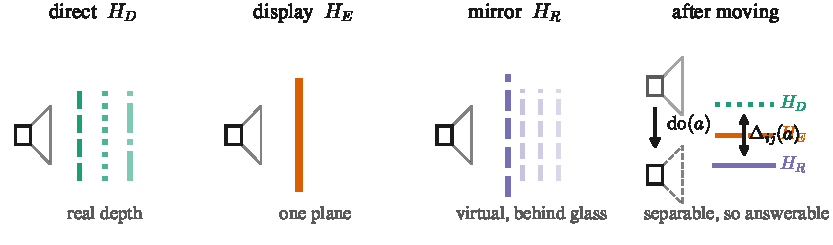
\includegraphics[width=0.92\linewidth]{figures/fig_concept.pdf}
\end{center}
\caption{\textbf{One image, three mechanisms, and what motion reveals.} A real
corridor, the same corridor painted on a display, and its virtual image in a
mirror can be arranged to produce identical pixels at the reference view, so no
single-view method separates them. They differ in the surface a hand would touch,
shown as the coloured plane in each panel. Executing an action makes their
predictions diverge, and the size of that divergence is the separability
$\Delta_{ij}(a)$ of \eqref{eq:separability}.}
\label{fig:concept}
\end{figure}

\section{The decision pipeline}
\label{sec:supp-pipeline}

\begin{figure}[!ht]
\begin{center}
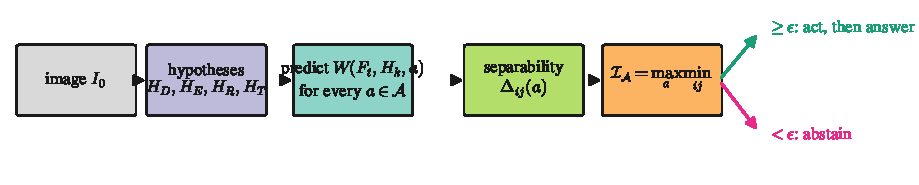
\includegraphics[width=0.96\linewidth]{figures/fig_pipeline.pdf}
\end{center}
\caption{\textbf{How the pieces compose.} Each hypothesis predicts the consequence
of every permitted action \eqref{eq:transition}; pairwise separabilities
\eqref{eq:separability} are formed from those predictions; identifiability is the
best value the action set attains on the weakest contending pair
\eqref{eq:identifiability}. Only when it clears the perceptual threshold is an
action executed and an answer given, and otherwise the system declines
\eqref{eq:abstain}. The whole comparison is made before any motion, which is what
allows abstention in advance of acting.}
\label{fig:pipeline}
\end{figure}

\section{The real-photograph protocol in detail}
\label{sec:supp-protocol}

\begin{figure}[!ht]
\begin{center}
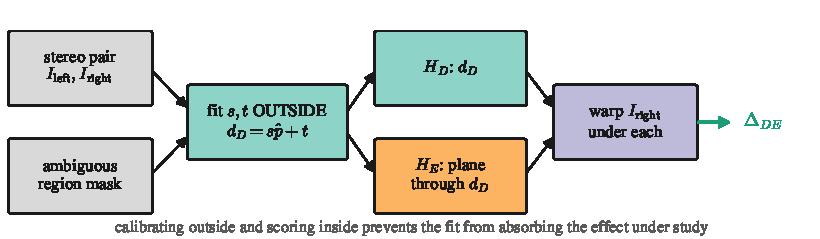
\includegraphics[width=\linewidth]{figures/fig_supp_protocol.pdf}
\end{center}
\caption{\textbf{Construction of the real-data measurement.} Scale and shift are
fitted on the non-ambiguous region and applied inside it, so the two free
parameters are determined where the predictor performs well and cannot absorb the
discrepancy in the region under study. Both hypotheses are then generated from the
predictor's own aligned disparity, never from the reference measurement, and the
right image is warped into the left frame under each. Comparing the two warps
rather than either against the opposite view cancels illumination, sensor noise and
rectification error, which appear identically in both.}
\label{fig:supp-protocol}
\end{figure}

\section{Minimum causal resolving baseline}
\label{sec:supp-mcrb}

For the pair consisting of a direct scene and a static planar display, the motion
required to separate them has a closed form. Under a lateral translation of
baseline $B$, a point at depth $Z$ shifts in the image by approximately $fB/Z$,
where $f$ is the horizontal focal length in pixels, so two points at depths
$Z_1 \neq Z_2$ produce a differential parallax of $fB\,|1/Z_1 - 1/Z_2|$. A static
planar display produces none once the screen-plane homography is compensated.
Requiring the differential parallax to exceed the perceptual threshold $\delta$
gives
\begin{equation}
\label{eq:mcrb}
B_{\min} \;>\; \frac{\delta}{f\left|1/Z_1 - 1/Z_2\right|},
\end{equation}
where $\delta$ coincides with $\epsilon$ whenever the composite distance is
dominated by its motion term. Equation~\eqref{eq:mcrb} is valid only for pure
lateral translation without rotation, a pinhole camera, small baselines satisfying
$B \ll Z$, and this hypothesis pair alone. It does not apply to view-tracked
displays, which no baseline resolves, nor to mirrors, whose virtual scene carries
genuine parallax. These conditions are checked before the expression is evaluated,
so a violated assumption yields a missing prediction rather than a confident wrong
one.

\section{Calibrated deferral and imperfect execution}
\label{sec:supp-noise}

Two studies are reported here: split-conformal deferral on the real benchmark, and the effect of executing a chosen action imperfectly on the synthetic one.

\begin{table}[!ht]
\caption{\textbf{Executing the chosen action imperfectly, paired over $11$ seeds}
($\pm 1$~cm, $\pm 0.5^{\circ}$). Methods that take no action are unchanged at
exactly $0.0\%$, the check that perturbation cannot reach a method that does not
act. Among methods that do act, the hypothesis-blind proxy loses roughly half its
accuracy while ours loses $2.9\%$: actions chosen with a large separability margin
tolerate perturbation, and that margin is what \eqref{eq:maximin} maximises.}
\label{tab:noise}
\begin{center}
\footnotesize
\resizebox{\linewidth}{!}{%
\begin{tabular}{lcccc}
\toprule
\textbf{Method} & \textbf{Clean CEA} & \textbf{Perturbed CEA} & \textbf{Change} & \textbf{$t$} \\
\midrule
Passive multi-view (does not act) & $0.621$ & $0.621$ & $+0.0\%$ & --- \\
Generic NBV proxy   & $0.371$ & $0.192$ & $-48.4\%$ & $-14.05$ \\
Random intervention & $0.409$ & $0.291$ & $-29.0\%$ & $-10.64$ \\
Max-baseline        & $0.502$ & $0.478$ & $-4.7\%$  & $-3.68$ \\
\textbf{Ours}       & $0.560$ & $0.544$ & $\mathbf{-2.9\%}$ & $-3.05$ \\
\bottomrule
\end{tabular}}
\end{center}
\end{table}

\begin{table}[!ht]
\caption{\textbf{Split-conformal selective prediction, $296$ images, $400$
calibration splits per level.} Both signals meet their coverage guarantee at every
level, so neither procedure is broken and the separation appears entirely in
selective risk, which coverage does not constrain. Deferring on confidence tracks
the base rate and then worsens, reaching $76.6\%$; deferring on identifiability
lowers the failure rate at every level, to $54.4\%$ at its best.}
\label{tab:conformal}
\begin{center}
\footnotesize
\resizebox{\linewidth}{!}{%
\begin{tabular}{lccccccc}
\toprule
& & \multicolumn{4}{c}{\textbf{Failure rate among retained images}} & & \\
\cmidrule(lr){3-6}
\textbf{Deferral signal} & \textbf{AUROC} & $\alpha{=}0.2$ & $\alpha{=}0.3$ &
$\alpha{=}0.4$ & $\alpha{=}0.5$ & \textbf{Coverage} & \textbf{Best gain} \\
\midrule
No abstention            & ---     & \multicolumn{4}{c}{$65.2\%$} & --- & --- \\
Confidence (TTA)         & $0.339$ & $64.2\%$ & $65.8\%$ & $69.2\%$ & $76.6\%$ & $5/5$ & $-1.0$ \\
\textbf{Identifiability} & $\mathbf{0.632}$ & $57.9\%$ & $55.1\%$ & $\mathbf{54.4\%}$ & $56.2\%$ & $5/5$ & $\mathbf{-10.8}$ \\
\bottomrule
\end{tabular}}
\end{center}
\end{table}


\section{Per-checkpoint results}
\label{sec:supp-models}

Table~\ref{tab:models} gives the per-checkpoint values summarised in Section~\ref{sec:res-universal}, with parameter counts and family membership.

\begin{table}[!ht]
\caption{\textbf{Twelve published checkpoints, six families, used as released.}
Every checkpoint is fooled on $59.5$--$78.4\%$ of admissible images, and the range
narrows neither with parameter count nor with recency. On every checkpoint the
model's own confidence scores \emph{below chance} at predicting its own failure, so
the usual deferral rule is inverted with respect to what it should track.
Confidence is the better of raw confidence and a four-member test-time-augmentation
ensemble.}
\label{tab:models}
\begin{center}
\footnotesize
\resizebox{\linewidth}{!}{%
\begin{tabular}{llrccc}
\toprule
\textbf{Checkpoint} & \textbf{Family} & \textbf{Params} & \textbf{Fooled} &
\textbf{Confidence AUROC} & \textbf{Ident.\ AUROC} \\
\midrule
DA-V2-Small     & Depth-Anything-V2 & $24.8$M  & $65.2\%$ & $0.344$ & $0.645$ \\
DA-V2-Base      & Depth-Anything-V2 & $97.5$M  & $67.2\%$ & $0.408$ & $0.588$ \\
DA-V2-Large     & Depth-Anything-V2 & $335.3$M & $66.6\%$ & $0.367$ & $0.467$ \\
DA-transparency & Depth-Anything-V2 & $24.8$M  & $\mathbf{59.5\%}$ & $\mathbf{0.234}$ & $0.719$ \\
DA3-Small       & Depth-Anything-3  & $24.8$M  & $76.4\%$ & $0.465$ & $0.479$ \\
DA3-Base        & Depth-Anything-3  & $97.5$M  & $68.2\%$ & $0.362$ & $0.576$ \\
DA3-Large       & Depth-Anything-3  & $410.9$M & $\mathbf{78.4\%}$ & $0.399$ & $0.512$ \\
DepthPro        & DepthPro          & $952.0$M & $65.2\%$ & $0.328$ & $0.659$ \\
MoGe-2          & MoGe-2            & $330.9$M & $62.2\%$ & $0.334$ & $0.642$ \\
Metric3D-Small  & Metric3D          & $37.5$M  & $64.5\%$ & $0.323$ & $0.593$ \\
Metric3D-Large  & Metric3D          & $343.0$M & $67.6\%$ & $0.406$ & $0.593$ \\
UniDepth-v2     & UniDepth          & $353.8$M & $66.2\%$ & $0.295$ & $0.692$ \\
\midrule
\emph{range} & \emph{6 families} & $38\times$ & $59.5$--$78.4\%$ & $0.234$--$0.465$ & $0.467$--$0.719$ \\
\bottomrule
\end{tabular}}
\end{center}
\end{table}

\section{Extended results by architecture family}
\label{sec:supp-family}

Averaging within architecture family confirms that the pattern is not driven by one lineage.

\begin{figure}[!ht]
\begin{center}
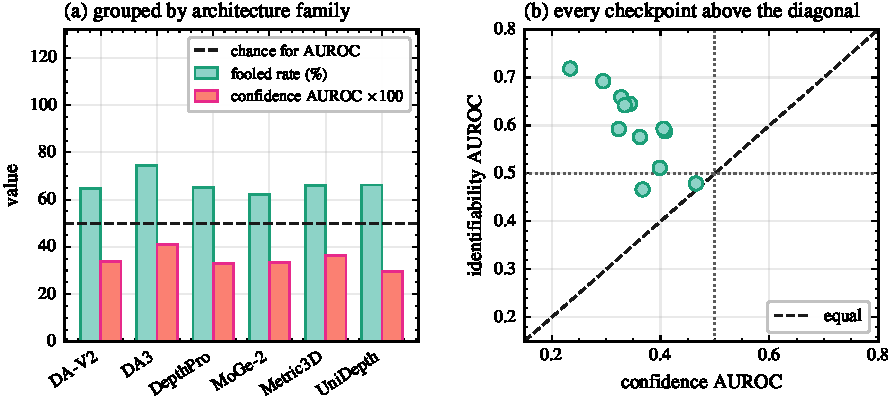
\includegraphics[width=\linewidth]{figures/fig_supp_extended.pdf}
\end{center}
\caption{\textbf{Grouped and paired views of Table~\ref{tab:models}.} (a) Averaged
within each architecture family, the fooled rate sits well above the confidence
AUROC in every family, and every family's confidence average falls below chance.
(b) The same twelve checkpoints plotted against one another: each point lies above
the diagonal, so identifiability exceeds confidence on every checkpoint without
exception, and every point lies to the left of the vertical chance line.}
\label{fig:supp-extended}
\end{figure}

\begin{table}[!ht]
\caption{\textbf{Per-family summary of the twelve checkpoints}, averaged within
family. The pattern of Table~\ref{tab:models} is not driven by one lineage: every
family is fooled on roughly two images in three, and every family's mean confidence
AUROC lies below chance.}
\label{tab:supp-family}
\begin{center}
\footnotesize
\resizebox{\linewidth}{!}{%
\begin{tabular}{lcccc}
\toprule
\textbf{Family} & \textbf{Checkpoints} & \textbf{Mean fooled} &
\textbf{Mean confidence} & \textbf{Mean identifiability} \\
\midrule
Depth-Anything-V2 & $4$ & $64.6\%$ & $0.338$ & $0.605$ \\
Depth-Anything-3  & $3$ & $74.3\%$ & $0.409$ & $0.522$ \\
DepthPro          & $1$ & $65.2\%$ & $0.328$ & $0.659$ \\
MoGe-2            & $1$ & $62.2\%$ & $0.334$ & $0.642$ \\
Metric3D          & $2$ & $66.1\%$ & $0.365$ & $0.593$ \\
UniDepth          & $1$ & $66.2\%$ & $0.295$ & $0.692$ \\
\midrule
\textbf{All}      & $\mathbf{12}$ & $\mathbf{67.3\%}$ & $\mathbf{0.355}$ & $\mathbf{0.597}$ \\
\bottomrule
\end{tabular}}
\end{center}
\end{table}

\section{Learned abstention, summary}
\label{sec:supp-learned}

The table below is the summary referred to from Section~\ref{sec:res-learned}; the section after it expands the leave-one-model-out column to every held-out checkpoint.

\begin{table}[!ht]
\caption{\textbf{Learned abstention.} Folds are split by base scene, so frames of
one scene never span a partition. Success under leave-one-model-out means a
property of the image was learned rather than of one predictor.}
\label{tab:supp-learned}
\begin{center}
\footnotesize
\begin{tabular}{lccc}
\toprule
\textbf{Policy} & \textbf{Grouped CV} & \textbf{Nested CV} & \textbf{Leave-one-model-out} \\
\midrule
\multicolumn{4}{l}{\emph{all 12 checkpoints, 3{,}552 image--model pairs, 68 scenes}} \\
Strongest single feature    & $0.762$ & --- & $0.764$ \\
Logistic regression         & $0.787$ & $0.748$ & $0.808$ \\
\textsc{XGBoost}            & --- & $0.832$ & --- \\
Histogram gradient boosting & $\mathbf{0.832}$ & $\mathbf{0.834}$ & $\mathbf{0.880}$ ($12/12$) \\
\midrule
\multicolumn{4}{l}{\emph{single checkpoint, identical data for all three}} \\
Strongest single feature    & $0.819$ & --- & --- \\
Hand-designed features      & $0.858$ & --- & --- \\
\textbf{Frozen-encoder head} & $\mathbf{0.879}$ & --- & --- \\
\bottomrule
\end{tabular}
\end{center}
\end{table}

\section{Full leave-one-model-out results}
\label{sec:supp-lomo}

The leave-one-model-out protocol of Table~\ref{tab:supp-learned} is expanded to every held-out checkpoint below, together with the regularisation sweep for the frozen-encoder head.

\begin{table}[!ht]
\caption{\textbf{Learned abstention in full.} \emph{Upper block:} every held-out
checkpoint from Table~\ref{tab:supp-learned}. The policy is trained on the other eleven
and evaluated on the one named, which it has never seen; it exceeds the strongest
single feature on all twelve, with a mean margin of $+0.115$ and a minimum of
$+0.051$. \emph{Lower block:} the frozen-encoder head against regularisation
strength. It varies by $0.026$ across three decades and exceeds the hand-designed
feature set ($0.858$) at every setting, so the result reflects the representation
rather than the choice of constant.}
\label{tab:supp-lomo}
\begin{center}
\footnotesize
\resizebox{\linewidth}{!}{%
\begin{tabular}{lccc|lccc}
\toprule
\textbf{Held out} & \textbf{Learned} & \textbf{Baseline} & \textbf{$\Delta$} &
\textbf{Held out} & \textbf{Learned} & \textbf{Baseline} & \textbf{$\Delta$} \\
\midrule
DA-V2-Small     & $0.917$ & $0.819$ & $+0.098$ & DA3-Large      & $0.837$ & $0.731$ & $+0.106$ \\
DA-V2-Base      & $0.901$ & $0.748$ & $+0.153$ & DepthPro       & $0.854$ & $0.721$ & $+0.133$ \\
DA-V2-Large     & $0.930$ & $0.812$ & $+0.118$ & MoGe-2         & $0.899$ & $0.756$ & $+0.143$ \\
DA-transparency & $0.842$ & $0.791$ & $+0.051$ & Metric3D-Small & $0.915$ & $0.787$ & $+0.128$ \\
DA3-Small       & $0.870$ & $0.781$ & $+0.089$ & Metric3D-Large & $0.858$ & $0.750$ & $+0.108$ \\
DA3-Base        & $0.887$ & $0.739$ & $+0.147$ & UniDepth-v2    & $0.849$ & $0.738$ & $+0.111$ \\
\midrule
\multicolumn{8}{c}{\textbf{mean} $\;0.880$ against $0.764$, margin $+0.115$, ahead on $12/12$} \\
\midrule
\multicolumn{8}{l}{\emph{frozen-encoder head: AUROC against regularisation strength $C$, grouped five-fold, one checkpoint}} \\
$C$ & $0.001$ & $0.005$ & $0.020$ & $0.100$ & $0.500$ & $2.000$ & $10.000$ \\
AUROC & $0.869$ & $0.878$ & $\mathbf{0.879}$ & $0.872$ & $0.864$ & $0.859$ & $0.853$ \\
\bottomrule
\end{tabular}}
\end{center}
\end{table}


\section{Per-category behaviour on the illusion benchmark}
\label{sec:supp-category}

The aggregate error ratio quoted in Section~\ref{sec:res-universal} resolves into three categories that behave quite differently.

\begin{table}[!ht]
\caption{\textbf{Admissible images by illusion category.} The penalty for reporting
depicted rather than physical geometry is largest where a display fills the frame,
and the reference measurement inside these regions is close to perfectly planar
while the prediction is not, confirming that the surface is flat and the prediction
is not. This is the per-category detail behind the aggregate quoted in
Section~\ref{sec:res-universal}.}
\label{tab:supp-category}
\begin{center}
\footnotesize
\resizebox{\linewidth}{!}{%
\begin{tabular}{lcccc}
\toprule
\textbf{Category} & \textbf{Images} & \textbf{Error ratio inside/outside} &
\textbf{Fooled} & \textbf{Reference planarity} \\
\midrule
Printed sheet on a table & $97$ & $0.78\times$ & $33\%$ & $0.99$ \\
Poster beside an object  & $104$ & $1.47\times$ & $63\%$ & $0.99$ \\
Monitor filling the frame & $95$ & $\mathbf{2.23\times}$ & $\mathbf{100\%}$ & $0.99$ \\
\midrule
\textbf{All admissible}  & $\mathbf{296}$ & $\mathbf{1.42\times}$ & $\mathbf{65.2\%}$ & $\mathbf{0.989}$ \\
\bottomrule
\end{tabular}}
\end{center}
\end{table}

\section{Second dataset with ordinal supervision}
\label{sec:supp-layered}

The second dataset supplies ordinal relations between point pairs rather than dense depth, and carries a per-point layer index authored independently of this work.

\begin{table}[!ht]
\caption{\textbf{LayeredDepth validation, $299$ images, $306{,}874$ annotated point
pairs.} Accuracy is split by the benchmark authors' own per-point layer index, a
label written independently of this work that shares no machinery with any measure
defined here. Both architectures are markedly worse on points visible only through
a transparent surface, and the penalty is larger for the model with more
parameters. The ambiguity this paper formalises is therefore recognised by an
independent annotation and independently predicts failure, on supervision that is
ordinal rather than dense and on a dataset collected by a different group.}
\label{tab:supp-layered}
\begin{center}
\footnotesize
\resizebox{\linewidth}{!}{%
\begin{tabular}{lccccc}
\toprule
\textbf{Checkpoint} & \textbf{Single-layer acc.} & \textbf{Multi-layer acc.} &
\textbf{Gap} & \textbf{Ordinal acc.\ (first surface)} & \textbf{Ordinal acc.\ (through glass)} \\
\midrule
DA-V2-Small & $0.848$ & $0.737$ & $\mathbf{+0.111}$ & $0.847$ & $0.784$ \\
DepthPro    & $0.843$ & $0.669$ & $\mathbf{+0.175}$ & $0.842$ & $0.741$ \\
\bottomrule
\end{tabular}}
\end{center}
\end{table}

\section{Choosing where to look}
\label{sec:supp-viewpoint}

Fifty-five non-video scenes offer three or more camera positions of the same
static content. Video scenes are excluded because their frames differ by what is
displayed rather than by where the observer stands, so treating them as an action
set would count a change of stimulus as a change of viewpoint.

\begin{table}[!ht]
\caption{\textbf{Viewpoint selection on real photographs}, $12$ checkpoints over
$55$ scenes, lower is better on both columns. Selecting by
\eqref{eq:evidence-selection}, the viewpoint at which some hypothesis best accounts
for the observed view, lowers the error inside the ambiguous region by $31.6\%$
against a random choice and wins on every checkpoint. Error inside the region is
the primary column because it depends on no other part of the image; the fooled
rate is reported alongside for continuity with the rest of the paper.}
\label{tab:supp-viewpoint}
\begin{center}
\footnotesize
\begin{tabular}{lcc}
\toprule
\textbf{Viewpoint chosen by} & \textbf{Error inside region} & \textbf{Fooled} \\
\midrule
first frame, no choice          & $0.0695$ & $49.2\%$ \\
uniformly at random             & $0.0610$ & $48.7\%$ \\
the predictor's own confidence  & $0.0450$ & $47.1\%$ \\
\textbf{best-explained observation} \eqref{eq:evidence-selection} & $\mathbf{0.0417}$ & $\mathbf{44.1\%}$ \\
\midrule
\multicolumn{3}{l}{\emph{ahead of a random choice on $12/12$ checkpoints by error, $9/12$ by fooled rate}} \\
\bottomrule
\end{tabular}
\end{center}
\end{table}

A note on the comparison with published methods. The benchmark's authors release
both their data and a trained checkpoint. The datasets carry an explicit
Apache-2.0 licence and are used here accordingly; the checkpoint carries no licence
field on its model repository, no \texttt{LICENSE} file on either default branch of
the source repository, and no licence statement in its README, all checked on
2026-08-29. A direct comparison against it is therefore deferred until those terms
are stated, rather than made under unclear ones.

\section{Metric definitions}
\label{sec:supp-metrics}

The metrics used throughout are defined below.

\begin{table}[!ht]
\caption{\textbf{The reported metrics.} $\hat{H}$ is the predicted mechanism,
$H^\star$ the true one, $p(H_k)$ the posterior mass on hypothesis $k$, $\tau$ the
confidence threshold of Section~\ref{sec:belief}, and $y_{\mathrm{id}} = 0$ marks a
case no permitted action resolves. CEA and committed accuracy are reported together
because the first penalises excessive caution and the second rewards it.}
\label{tab:supp-metrics}
\begin{center}
\footnotesize
\begin{tabular}{llp{6.0cm}}
\toprule
\textbf{Metric} & \textbf{Definition} & \textbf{Question it answers} \\
\midrule
CEA & $P(\hat{H} = H^\star)$ & how often the mechanism is named correctly, abstention counted as an error \\
Committed acc. & $P(\hat{H} = H^\star \mid \text{answered})$ & when an answer is given, how often it is right \\
Abstention rate & $P(\text{abstain})$ & how often an answer is withheld \\
FPCR & $P(\max_k p(H_k) > \tau \mid y_{\mathrm{id}} = 0)$ & how often a confident answer is given where none is warranted \\
Ident.\ AUROC & predicted against true resolvability & whether unresolvable cases are recognised \\
Normalised regret & chosen against best available action & whether a near-optimal intervention was selected \\
Motion cost & translation plus weighted rotation & how much movement the decision required \\
\bottomrule
\end{tabular}
\end{center}
\end{table}

\section{Scope and limitations}
\label{sec:supp-limits}

Four limits bound what the reported numbers establish, and each is visible in the
results rather than inferred.

\textbf{The synthetic identifiability AUROC is degenerate by construction.} On the
synthetic benchmark the computation producing the identifiability prediction is the
same one producing the ground-truth label, so the value of $1.000$ in
Table~\ref{tab:phase1} carries no information about the method's accuracy. It is
reported only as a contrast against the classifiers, which reach $0.505$ and
$0.748$ on identical scenes, and no claim rests on its absolute value.

\textbf{Abstention is not unconditionally safe under encoder noise.} The clean
configuration reaches a false physical certainty rate of $0.000 \pm 0.000$ across
all $11$ seeds, but the noisy-encoder ablation reaches $0.008 \pm 0.026$: one seed
in eleven produces a false certainty. The correct statement is therefore
``zero in $10$ of $11$ seeds under encoder noise'', not ``zero''.

\textbf{Real-data evidence rests on stereo, which supplies a single action.} A
calibrated pair gives $|\mathcal{A}| = 1$, so \eqref{eq:identifiability} reduces to
one term and the selection results of Table~\ref{tab:phase2} cannot be tested on
this data. Evaluating the choice of intervention on real photographs requires a
multi-view or controllable-camera capture, which the datasets used here do not
provide.

\textbf{One checkpoint runs in a degraded configuration.} UniDepth-v2 has no
optimised attention kernel for the available hardware and falls back to a slower
path, so its numbers in Table~\ref{tab:models} are a lower bound on the released
model rather than a tuned comparison. It is retained because excluding a checkpoint
on the basis of its result would bias the sweep.

\section{Reproducibility}
\label{sec:supp-repro}

All synthetic results are averaged over $11$ seeds with the benchmark redrawn per
seed, so the reported intervals reflect the data-generating process rather than
model-side noise alone. Splits are formed by base scene throughout, in both the
synthetic benchmark and the learned-policy protocols, so variants or frames of a
single scene never span a partition. Every depth checkpoint is used exactly as
released and nothing is trained or tuned on any evaluation set. Each checkpoint's
output convention is verified against reference stereo disparity before use, since
the attribute conventionally named \texttt{predicted\_depth} carries metric depth
in some families and inverse depth in others. One checkpoint, UniDepth-v2, runs
without its optimised attention kernel on the available hardware, so its numbers
should be read as a lower bound on the released model rather than a tuned
comparison.


\end{document}
